\section{Attività di verifica}
Si analizzano qui le metriche:
\begin{itemize}
    \item \hyperref[s:mpc02]{\textbf{MPC02}}\textbf{}: \textit{Budget Variance}.
    \item \hyperref[s:mpc04]{\textbf{MPC04}}\textbf{}: \textit{Budgeted Cost of Work Scheduled}.
    \item \hyperref[s:mpc06]{\textbf{MPC06}}\textbf{}: \textit{Actual Cost of Work Performed}.
    \item \hyperref[s:mpc07]{\textbf{MPC07}}\textbf{}: \textit{Requirements stability index}.
    \item \hyperref[s:mpc08]{\textbf{MPC08}}\textbf{}: \textit{Satisfied obligatory requirements}.
    \item \hyperref[s:mpd1]{\textbf{MPD1}}\textbf{}: Indice di Gulpease.
    \item \hyperref[s:mpd1]{\textbf{MPD2}}\textbf{}: Copertura dei requisiti.
\end{itemize}

\subsection{MPC02 - Budget Variance}
\label{s:mpc02}
La \textit{Budget Variance} confronta il costo effettivo del lavoro completato fino a un certo punto nel tempo con il costo pianificato per quel lavoro.
Il valore negativo riportato in Figura \ref{fig:mpc02} indica che il costo effettivo è superiore al \textit{budget} pianificato.
Il valore medio riportato rientra nel margine di accettabilità stabilito. \\
Il gruppo ritiene che, nella prima fase RTB, lo sforamento del \textit{budget} sia dovuto alla generale inesperienza dei vari membri nella gestione di un progetto e nell'uso delle tecnologie, che ha portato alla necessità di incrementare il tempo di lavoro.\\
Nella seconda fase il gruppo ha individuato delle problematiche che non erano note nella fase precedente, questo grazie all'esperienza maturata durante lo sviluppo.
Tali problematiche hanno aumentato le attività da svolgere per mettere in atto operazioni di correzione, questo ha portato ad uno sforamento del \textit{budget}.
In particolare durante il sesto \textit{sprint}, il gruppo si è reso conto di aver sottostimato le ore necessarie per svolgere le attività di programmazione.
La pianificazione del lavoro negli \textit{sprint} successivi è stata quindi rivista adeguando le ore necessarie alla programmazione con quandto sperimentato nello \textit{sprint} numero 6.

\begin{figure}[htbp]
    \centering
    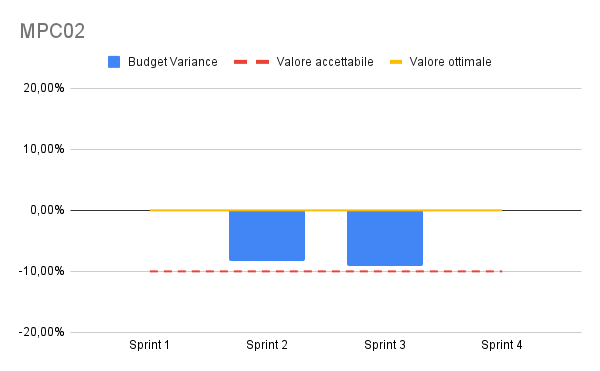
\includegraphics[width=0.8\textwidth]{img/MPC02.png}
    \caption{MPC02 - Budget Variance}
    \label{fig:mpc02}
\end{figure}


\newpage

\subsection{MPC04 - Budgeted Cost of Work Scheduled}
\label{s:mpc04}
Rappresenta il costo del lavoro pianificato per essere completato entro una data specifica nel progetto.\\
Nel grafico in Figura \ref{fig:mpc04} è stato inserito anche il costo relativo ad ogni \textit{sprint} al fine di indicare più intuitivamente il contributo di ogni singola fase al costo complessivo.\\
Il minor costo associato al quarto \textit{sprint} deriva dalla necessità di ridurre le ore di lavoro utile in concomitanza dei numerosi impegni, sia personali che legati alla sessione di esami, dei membri del gruppo.\\
Il consumo di risorse, confrontato con il preventivo dei costi presente nel documento \href{https://project-swenergy.github.io/Candidatura/Presentazione%20costi%20e%20assunzione%20impegni.pdf}{Presentazione costi ed assunzione impegni v2.0.0}, risulta ragionevole in considerazione della diversa durata delle fasi RTB e PB.\\
A partire dalla fase PB, relativa allo \textit{sprint} numero 5, si ha una crescita lineare costante che indica:
\begin{itemize}
    \item \textbf{Stima accurata}: le stime iniziali per il progetto sono precise e il lavoro si sta svolgendo secondo la pianificazione senza grandi variazioni o imprevisti.
    \item \textbf{Stabilità del processo}: indica che il processo utilizzato per completare il lavoro è stabile e prevedibile.
    \item \textbf{Controllo del progetto}: indica che il progetto è ben gestito e che ci sono processi di controllo efficaci per monitorare il progresso e intervenire tempestivamente in caso di deviazioni dalla pianificazione.
\end{itemize}
Le problematiche riscontrate durante lo sviluppo sono quindi state correttamente gestite per consentire un progresso lineare e, quindi, più facilmente gestibile.

\begin{figure}[htbp]
    \centering
    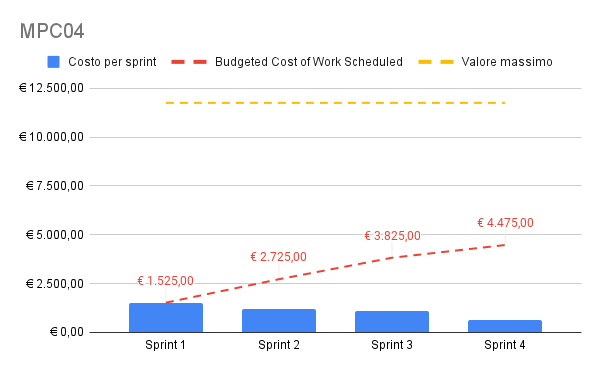
\includegraphics[width=0.7\textwidth]{img/MPC04.png}
    \caption{MPC04 - Budgeted Cost of Work Scheduled}
    \label{fig:mpc04}
\end{figure}



\subsection{MPC06 - Actual Cost of Work Performed}
\label{s:mpc06}
Il valore riportato in Figura \ref{fig:mpc06} indica che, a seguito del primo \textit{sprint}, il costo effettivo sostenuto ha superato quello preventivato.\\
Il gruppo ritiene che che il superamento del costo preventivato sia dovuto alla generale inesperienza dei vari membri nella gestione di un progetto e nell'uso delle tecnologie, che ha portato alla necessità di incrementare il tempo di lavoro nella fase iniziale del progetto.\\
Nonostante il superamento del valore ottimale, il costo effettivo è rimasto complessivamente all'interno del margine di accettabilità indicato nella metrica in esame.

\begin{figure}[htbp]
    \centering
    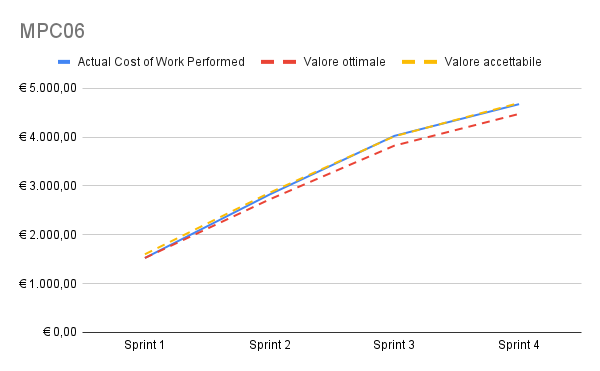
\includegraphics[width=0.7\textwidth]{img/MPC06.png}
    \caption{MPC06 - Actual Cost of Work Performed}
    \label{fig:mpc06}
\end{figure}


\subsection{MPC07 - Requirements stability index}
\label{s:mpc07}
Indica la stabilità dei requisiti nel corso del tempo.
Un RSI più alto indica una maggiore instabilità dei requisiti, mentre un RSI più basso indica una maggiore stabilità.
I requisiti sono stati aggiornati in seguito alla fase RTB, a seguito del dialogo con il proponente e alla presentazione del lavoro svolto.
Le modifiche apportate ai requisiti rientrano comunque all'interno del margine di accettabilità previsto.
\begin{table}[H]
    \centering
    \begin{tabularx}{\textwidth}{X|l|l|l|l}
        \hline
        \textbf{Metrica}             & \textbf{Codice} & \textbf{Valore ottimale} & \textbf{Valore accettabile} & \textbf{Valore attuale} \\
        \hline
        Requirements stability index & MPC07           & 0\%                      & 10\%                        & 8\%                  \\
    \end{tabularx}
\end{table}


\subsection{MPC08 - Satisfied obligatory requirements}
\label{s:mpc08}
Il numero di requisiti obbligatori è stato ridotto a seguito del colloquio avuto con il proponente nell'ottavo \textit{sprint}.
La necessità di ridurre il numero di requisiti obbligatori è stata causata dal ritardo accumulato nello sviluppo e dalla necessità di mantenere il più possibile invariata la data di consegna del progetto.
Al termine del nono \textit{sprint} sono stati soddisfatti tutti i requisiti obbligatori individuati.
\begin{table}[H]
    \centering
    \begin{tabularx}{\textwidth}{X|l|l|l|l}
        \hline
        \textbf{Metrica}                  & \textbf{Codice} & \textbf{Valore ottimale} & \textbf{Valore accettabile} & \textbf{Valore attuale} \\
        \hline
        Satisfied obligatory requirements & MPC08           & 100\%                    & 100\%                       & 100\%                   \\
    \end{tabularx}
\end{table}


\subsection{MPC09 - Non-calculated risk}
\label{s:mpc09}


\subsection{MPC10 - Code Coverage}
\label{s:mpc10}
\begin{table}[H]
    \centering
    \begin{tabularx}{\textwidth}{p{5.5cm}|X|l|l|l}
        \hline
        \textbf{Metrica} & \textbf{Codice} & \textbf{Valore ottimale} & \textbf{Valore accettabile} & \textbf{Valore attuale} \\
        \hline
        Code Coverage    & MPC10           & $100\%$                  & $\ge 80\%$                  &                         \\
    \end{tabularx}
\end{table}


\subsection{MPC11 - Passed Test Cases Percentage}
\label{s:mpc11}
\begin{table}[H]
    \centering
    \begin{tabularx}{\textwidth}{p{5.5cm}|X|l|l|l}
        \hline
        \textbf{Metrica}             & \textbf{Codice} & \textbf{Valore ottimale} & \textbf{Valore accettabile} & \textbf{Valore attuale} \\
        \hline
        Passed Test Cases Percentage & MPC11           & $100\%$                  & $\ge 100\%$                 &                         \\
    \end{tabularx}
\end{table}




\subsection{MPD1 - Indice di Gulpease}
\label{s:mpd1}
Il grafico in Figura \ref{fig:mpd1} mostra un miglioramento nella leggibilità media dei documenti redatti, avvenuto a seguito della fase di Candidatura.\\
Questo miglioramento è dovuto alla definizione di metriche di qualità che hanno portato il gruppo a prestare maggiore attenzione durante la scrittura della documentazione.
Il valore medio dell'indice di Gulpease ha così superato, per la fase RTB, la soglia di accettabilità.

\begin{figure}[htbp]
    \centering
    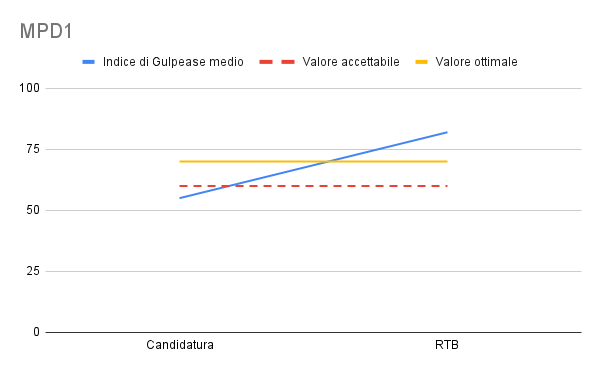
\includegraphics[width=0.7\textwidth]{img/MPD1.png}
    \caption{MPD1 - Indice di Gulpease}
    \label{fig:mpd1}
\end{figure}



\subsection{MPD2 - Copertura dei requisiti}
\label{s:mpd2}
\begin{table}[H]
    \centering
    \begin{tabularx}{\textwidth}{X|X|l|l|l}
        \hline
        \textbf{Metrica}        & \textbf{Codice} & \textbf{Valore ottimale} & \textbf{Valore accettabile} & \textbf{Valore attuale} \\
        \hline
        Copertura dei requisiti & MPD2            & $100\%$                  & $80\%$                      & $71,2\%$                \\
        \hline
    \end{tabularx}
\end{table}
Non è stato possibile raggiungere il valore ottimale di copertura dei requisiti.\\
Durante la fase PB il gruppo si è reso conto, approfondendo la conoscenza delle tecnologie utilizzate, di aver sottostimato il tempo necessario per l'implementazione delle funzionalità previste all'inizio del progetto.
Questo ha portato ad una ristrutturazione del documento Analisi dei requisiti, riducendo il numero di requisiti obbligatori presenti.
Siccome le ore di lavoro disponibili sono rapidamente state consumate per le attività di codifica, il gruppo ha scelto di non soddisfare parte dei requisiti non obbligatori, preferendo non ritardare la data di consegna del progetto.
